% Template for ICASSP-2018 paper; to be used with:
%          spconf.sty  - ICASSP/ICIP LaTeX style file, and
%          IEEEbib.bst - IEEE bibliography style file.
% --------------------------------------------------------------------------
\documentclass{article}
\usepackage{spconf,amsmath,graphicx,cite}

% Example definitions.
% --------------------
\def\x{{\mathbf x}}
\def\L{{\cal L}}

\usepackage[x11names]{xcolor}
\newif\ifproofread

\newcommand{\pfmarker}[1]{%
\ifproofread
\textcolor{red}{#1}%
\else
#1%
\fi
}
\proofreadtrue

% Title.
% ------
\title{SEMI-SUPERVISED LEARNING WITH DEEP NEURAL NETWORKS\\FOR RELATIVE TRANSFER FUNCTION INVERSE REGRESSION }
%
% Single address.
% ---------------
%\name{Author(s) Name(s)\thanks{Thanks to XYZ agency for funding.}}
%\address{Author Affiliation(s)}
%
% For example:
% ------------
%\address{School\\
%	Department\\
%	Address}
%
% Two addresses (uncomment and modify for two-address case).
% ----------------------------------------------------------
\twoauthors
  {Ziteng Wang\sthanks{We thank CSC (201604910623) for funding. This work was performed while the author was at Inria. Experiments presented in this paper were carried out using the Grid'5000 testbed, supported by a scientific interest group hosted by Inria and including CNRS, RENATER and several Universities as well as other organizations (see \texttt{https://www.grid5000.fr}).}, Junfeng Li, Yonghong Yan}
	{ University of Chinese Academy of Sciences \\
 Institute of Acoustics, Beijing, China}
  {Emmanuel Vincent}
	{Inria\\
	F-54600 Villers-l{\`e}s-Nancy, France}
%
\begin{document}
\ninept
%
\maketitle
%
\begin{abstract}
Prior knowledge of the relative transfer function (RTF) is useful in many applications but remains little studied. In this paper, we propose a semi-supervised learning algorithm based on deep neural networks (DNNs) for RTF inverse regression, that is to generate the full-band RTF vector directly from the source-receiver pose (position and orientation). Two typical scenarios are discussed: training on labeled RTFs only, or on additional unlabeled RTFs. Both setups utilize the low-dimensional manifold property of RTF in stationary environments. With this property as an additional regularization term, a smooth mapping solution with respect to the manifold is obtained. Experimental simulations show that the proposed method achieves a lower mean prediction error than the free field model with few labeled RTFs, and the unlabeled RTFs are essential in improving the inverse regression performance.
\end{abstract}
%
\begin{keywords}
relative transfer function, semi-supervised learning, deep neural network, manifold regularization
\end{keywords}
%
\section{INTRODUCTION}
\label{sec:intro}

% v 1: background -> RTF->AIR modeling -> Supervised -> Semi-supervised
% v 2: background -> Supervised -> Semi-supervised

The relative transfer function (RTF)~\cite{gannot2001signal,cohen2004relative} represents the difference between the signals recorded at two microphones in response to a source signal. The estimation of the RTF is a core task in many applications, such as beamforming and multichannel speech enhancement~\cite{talmon2009relative,reindl2013stereo,gannot2017perspective}, source separation~\cite{araki2007underdetermined,sawada2007grouping,taseska2015relative}, and source localization~\cite{li2015estimation}. Generally the estimation is merely based on the microphone observations, and prior knowledge about the RTF given the geometry of the scene remains little studied and exploited. Yet such knowledge could bring additional performance benefits~\cite{talmon2013relative,koldovsky2013semi}.

The RTF is defined as the ratio of two acoustic transfer functions (ATFs) and hence depends on the properties of the acoustic environment and on the \emph{poses} (positions and orientations) of the source and the microphone pair. Conventional room acoustic simulation methods, such as the image-source method~\cite{allen1979image}, rely on explicit physical models to simulate the ATFs. They require precise knowledge of the room geometry and the absorption properties of each material, which is not available in real environments. In such environments, the problem can be reformulated as that of predicting the RTF for a given pose given a set of RTFs or ATFs recorded for other poses. Recent studies have performed ATF interpolation based on room geometry estimation~\cite{asaei2014structured}, compressed sensing~\cite{mignot2013room,mignot2014low} or models derived from the wave propagation equation~\cite{samarasinghe2015efficient}.

In~\cite{rtfinv2017}, we proposed to predict the full-band RTF vector from a distinctive data-driven perspective, which we coined as \emph{RTF inverse regression}. We trained a deep neural network (DNN) to map the low-dimensional source pose to the high-dimensional RTF. Training was performed in a supervised fashion, based on a set of RTFs and the corresponding poses collected in advance. It turned out that, with dense enough training samples (i.e., when the corresponding poses form a grid with less than 4~cm stepsize), simple linear interpolation~\cite{vincent2013second} achieves a low prediction error. However, the DNN achieves a lower error when the training samples are further apart, which is a more realistic setup.

Unless the training RTFs are collected by fully automated mobile robots \cite{leroux2015micbots}, labeling them all with the corresponding poses can be cumbersome in a real environment. In this paper, we propose to train the DNN in a semi-supervised way on a set of RTFs of which only few have been labeled with the corresponding pose. This setup is feasible in practice by, e.g., recording from a mobile phone or any other smart device worn by a human freely moving in the environment. As a matter of fact, this setup is the core of a recent series of studies on audio source localization \cite{laufer2016mr}. To train on the unlabeled RTFs, we propose an \emph{encoder-decoder} framework and utilize the low-dimensional manifold property of RTFs \cite{deleforge20122d,laufer2013relative,deleforge2015acoustic}. Specifically, we introduce a smoothness constraint on the manifold to regularize the encoder network, which provides noisy labels for the unlabeled RTFs that are exploited together with the labeled RTFs to train the decoder network. We investigate the function and the benefit of the unlabeled RTFs experimentally. %The results show that the performance degrades with few labeled data compared to the fully labeled case, but the unlabeled samples are indispensable in the inverse regression performance.

The structure of the paper is as follows. We define notations in Section \ref{sec:defs} and summarize prior work on supervised RTF inverse regression in Section \ref{sec:prior}. We introduce the proposed semi-supervised encoder-decoder architecture in Section \ref{sec:inverse} and describe an alternative decoder architecture in Section \ref{sec:regul}. We evaluate the proposed method experimentally in Section \ref{sec:expe}. We conclude in Section \ref{sec:con}.


\section{DEFINITIONS}
\label{sec:defs}
Let us consider an unknown signal $S$ emitted from a source and captured by a pair of microphones in a fixed environment. For simplicity, we also assume the microphones to be fixed. The source pose is denoted as ${\bf p}=[\rho,\theta,\phi,\alpha,\beta,\gamma]$, with $\rho$, $\theta$, $\phi$ its distance, azimuth, and elevation with respect to the microphone pair and $\alpha$, $\beta$, $\gamma$ its yaw, pitch, and roll. In the short-time Fourier transform (STFT) domain, under the narrowband approximation, the signal $A_m(n,k)$ recorded at the $m$-th microphone can be written as
\begin{equation}\label{eq:sigfreq}
  A_m(n,k) = H_m({\bf p},k)S(n,k) + V_m(n,k),
\end{equation}
with $n$ the time frame index, $k$ the frequency bin index, $H_m({\bf p},k)$ the ATF from the source to the $m$-th microphone, and $V_m(n,k)$ sensor noise. The RTF $H({\bf p}, k)$ associated with source pose ${\bf p}$ is defined as
\begin{equation}\label{eq:rtf}
  H({\bf p}, k) = \frac{H_2({\bf p}, k)}{H_1({\bf p}, k)}.
\end{equation}

The RTF is independent of the source signal and, in a stationary environment, it depends only on the source pose. For instance, in a free-field environment, the relationship is given by
\begin{equation}\label{eq:green}
  H^\text{free-field}({\bf p},k)=\exp\left(2\jmath\pi \frac{k}{F}f_\text{s}\frac{|r_2({\bf p}) - r_1({\bf p})|}{c}\right),
\end{equation}
with $\jmath$ the complex unit, $F$ the discrete Fourier transform size, $f_\text{s}$ the sampling frequency, $c$ the speed of sound, and $r_m({\bf p})$ the Euclidean distance from the source to the $m$-th microphone. In a reverberant environment, this relationship becomes more complex due to multi-path propagation.

The RTF is often expressed via the interchannel level difference $\text{ILD}({\bf p}, k)=20\log_{10}|H({\bf p}, k)|$ and the interchannel phase difference $\text{IPD}({\bf p}, k)=\arg(H({\bf p}, k))$. In the following, we consider the $1\times 3K$ full-band RTF vector ${\bf h}$ obtained by concatenating the ILDs and the sines and cosines of the IPDs at all frequencies:
\begin{equation}
\label{eq:h}
\begin{aligned}
{\bf h}=&\left[\begin{matrix}\text{ILD}({\bf p}, 0) & \cdots & \text{ILD}({\bf p}, K-1)\end{matrix}\right.\\
&\qquad\begin{matrix}\sin(\text{IPD}({\bf p}, 0)) & \cdots & \sin(\text{IPD}({\bf p}, K-1))\end{matrix}\\
&\qquad\qquad\left.\begin{matrix}\cos(\text{IPD}({\bf p}, 0)) & \cdots & \cos(\text{IPD}({\bf p}, K-1))\end{matrix}\right]
\end{aligned}
\end{equation}
with $K=\frac{F}{2}+1$ the number of frequency bins.

We define RTF inverse regression as the problem of predicting the full-band RTF vector ${\bf h}$ from the source pose ${\bf p}$ based on pre-collected training examples, \pfmarker{and without making a measurement at that pose}. Using machine learning terminology, we refer to ${\bf h}$ as a \emph{sample} and to the corresponding pose ${\bf p}$ as a \emph{label}.


\section{SUPERVISED RTF INVERSE REGRESSION}
\label{sec:prior}
In~\cite{deleforge2015acoustic}, probabilistic piecewise affine mapping (PPAM) was used to learn a bijective mapping between ${\bf h}$\footnote{The authors used a slightly different representation of ${\bf h}$ by combining each $\sin(\text{IPD})$ and $\cos(\text{IPD})$ pair into a unit-norm complex number.} and ${\bf p}$ based on a set of $L$ labeled training samples $\{{\bf h}_{1:L}, {\bf p}_{1:L}\}$. However, this method was only applied to source localization (i.e., mapping ${\bf h}$ into ${\bf p}$).

In \cite{rtfinv2017}, we proposed to train a feedforward DNN $\mathcal{D}$ to directly map ${\bf p}$ into ${\bf h}$ by minimizing the mean square error (MSE) on the training set
\begin{equation}\label{eq:Dmmse}
  \text{MSE} = \sum_{i=1}^L\|\mathcal{D}({\bf p}_i) - {\bf h}_i\|^2
\end{equation}
where $\mathcal{D}({\bf p})$ denotes the DNN output RTF vector from the input pose ${\bf p}$. We used a specific output activation function that normalizes the output nodes $(o_{K+k},o_{2K+k})$ corresponding to each sine and cosine pair as
\begin{equation}\label{eq:ln}
  o_{K+k}\leftarrow \frac{o_{K+k}}{\sqrt{o_{K+k}^2+o_{2K+k}^2}}\quad\text{and}\quad o_{2K+k}\leftarrow \frac{o_{2K+k}}{\sqrt{o_{K+k}^2+o_{2K+k}^2}}
\end{equation}
such that their squared sum is always equal to 1 and they can indeed be interpreted as the sine and cosine of the predicted IPD. In the test phase, the trained DNN was used to generate the RTF of a new pose ${\bf p}_t$ as $\widehat{{\bf h}}_t=\mathcal{D}({\bf p}_t)$. This model is illustrated in Fig.~\ref{fig:dnn}(c).

In~\cite{rtfinv2017}, we evaluated PPAM in terms of RTF inverse regression performance and compared it with linear interpolation and the above DNN. These three methods are based on supervised training.


\section{SEMI-SUPERVISED RTF INVERSE REGRESSION}
\label{sec:inverse}
% why ILD/IPD
In the rest of this paper, we consider a semi-supervised setup: there are only $L$ labeled training samples $\{{\bf h}_{1:L}, {\bf p}_{1:L}\}$ and the remaining $U$ training samples $\{{\bf h}_{L+1:L+U}\}$ are unlabeled. To utilize the unlabeled samples in the training process, we propose an intuitive encoder-decoder architecture in Section \ref{subsec:archi}. We refine this idea in Section \ref{subsec:manifold} by optimizing the encoder network with manifold regularization. The proposed architectures are illustrated in Fig.~\ref{fig:dnn}. The network training details are discussed in Section \ref{subsec:train}.

\begin{figure}[tb]
    \centering
    \centerline{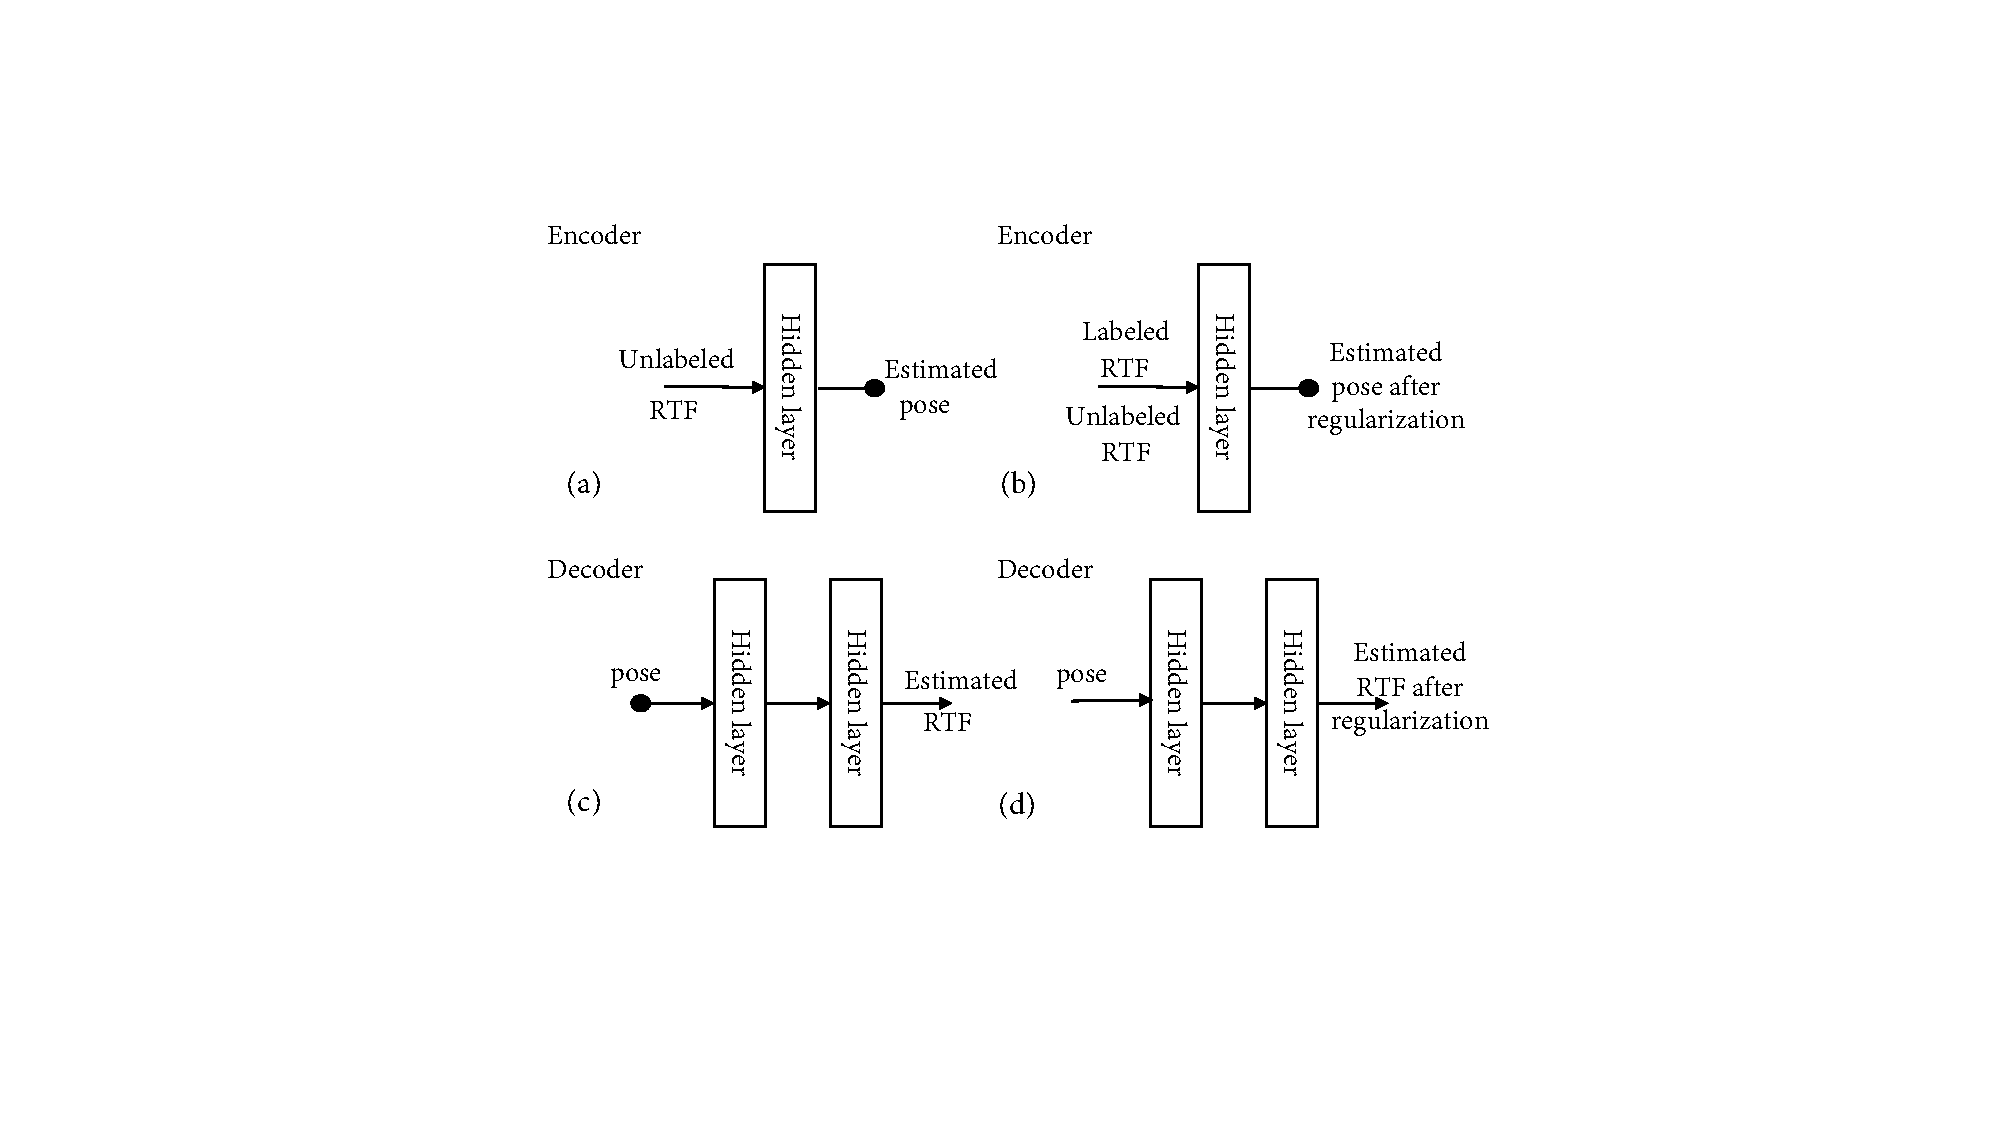
\includegraphics[width=8.3cm]{fig1_nn.pdf}}
    \caption{Proposed encoder and decoder networks for semi-supervised RTF inverse regression. The black dots indicate the connection points of the networks.}
    \label{fig:dnn}
\end{figure}

\subsection{Encoder-decoder architecture}
\label{subsec:archi}
We refer to the DNN in Section \ref{sec:prior} and Fig.~\ref{fig:dnn}(c) as the \emph{decoder} network. We introduce an auxiliary \emph{encoder} network $\mathcal{E}$ to help optimize the decoder network under the new loss function:
\begin{equation}\label{eq:lossed}
\sum_{i=1}^{L}\|\mathcal{D}({\bf p}_i)-{\bf h}_i\|^2 + \lambda \sum_{\pfmarker{j=L+1}}^{L+U}\|\mathcal{D}(\mathcal{E}({\bf h}_j))-{\bf h}_j\|^2
\end{equation}
where $\lambda$ is a constant scaling factor. The first term is the MSE \eqref{eq:Dmmse} on the labeled training samples and the second term is the reconstruction error on all training samples. This network architecture is given in Fig.~\ref{fig:dnn}(a)+(c). The encoder can be interpreted as a localization network, that maps the RTF space to the pose space and is expected to learn the pose labels implicitly. In the training phase, the encoder and decoder parameters are jointly updated to minimize \eqref{eq:lossed}.

\subsection{Encoder with manifold regularization}
\label{subsec:manifold}
Prior work on manifold regularization for audio source localization \cite{laufer2016mr} has shown that the RTFs in a given environment lie on a smooth low-dimensional manifold. A simple validation of this concept is shown in Fig.~2, that plots the Euclidean distance between full-band RTF vectors as a function of the difference between the corresponding source poses. Within a local area (about $\pm 1.6^\circ$ in azimuth and elevation in this example), the distance between the RTFs increases approximately linearly with azimuth and elevation difference and the slope is similar in all directions. In other words, a small shift in the source pose only leads to small changes in the RTF and vice-versa. The detailed setup can be found in Section \ref{sec:expe}.

Inspired by this property, we further refine the encoder network from a localization perspective under the loss function:
\begin{equation}\label{eq:lossmr}
\sum_{i=1}^{L}\|\mathcal{E}({\bf h}_i)-{\bf p}_i\|^2 + \mu \sum_{i=1}^{L+U}\sum_{j=1}^{L+U}W_{ij}\|\mathcal{E}({\bf h}_i)-\mathcal{E}({\bf h}_j)\|^2
\end{equation}
that incurs a weighted penalty when similar inputs have different outputs. $\mu$ is a scaling factor and the second term is commonly known as graph Laplacian regularization~\cite{Yang2016Revisiting}, that imposes a smoothness constraint on the final mapping solution. $W_{ij}$ is the weight that reflects the adjacency between encoder inputs ${\bf h}_i$ and ${\bf h}_j$, and it is close to 0 when the samples are far away. The standard Gaussian kernel function is used for weight calculation as in~\cite{laufer2016mr}, since it is symmetric positive semi-definite and meets the locality requirements:
\begin{equation}\label{eq:wij}
  W_{ij} = \exp\left(-\frac{\|{\bf h}_i-{\bf h}_j\|^2}{\varsigma^2}\right)
\end{equation}
where the variance $\varsigma^2$ controls how fast the weight decays with the distance between RTFs. Accordingly, the new encoder-decoder architecture is given in Fig.~\ref{fig:dnn}(b)+(c).

The encoder is first trained to minimize \eqref{eq:lossmr} and then kept fixed when the decoder is optimized under loss (\ref{eq:lossed}). Further joint tuning didn't bring additional performance gains in our experiments.

\begin{figure}[tb]
    \centering
    \centerline{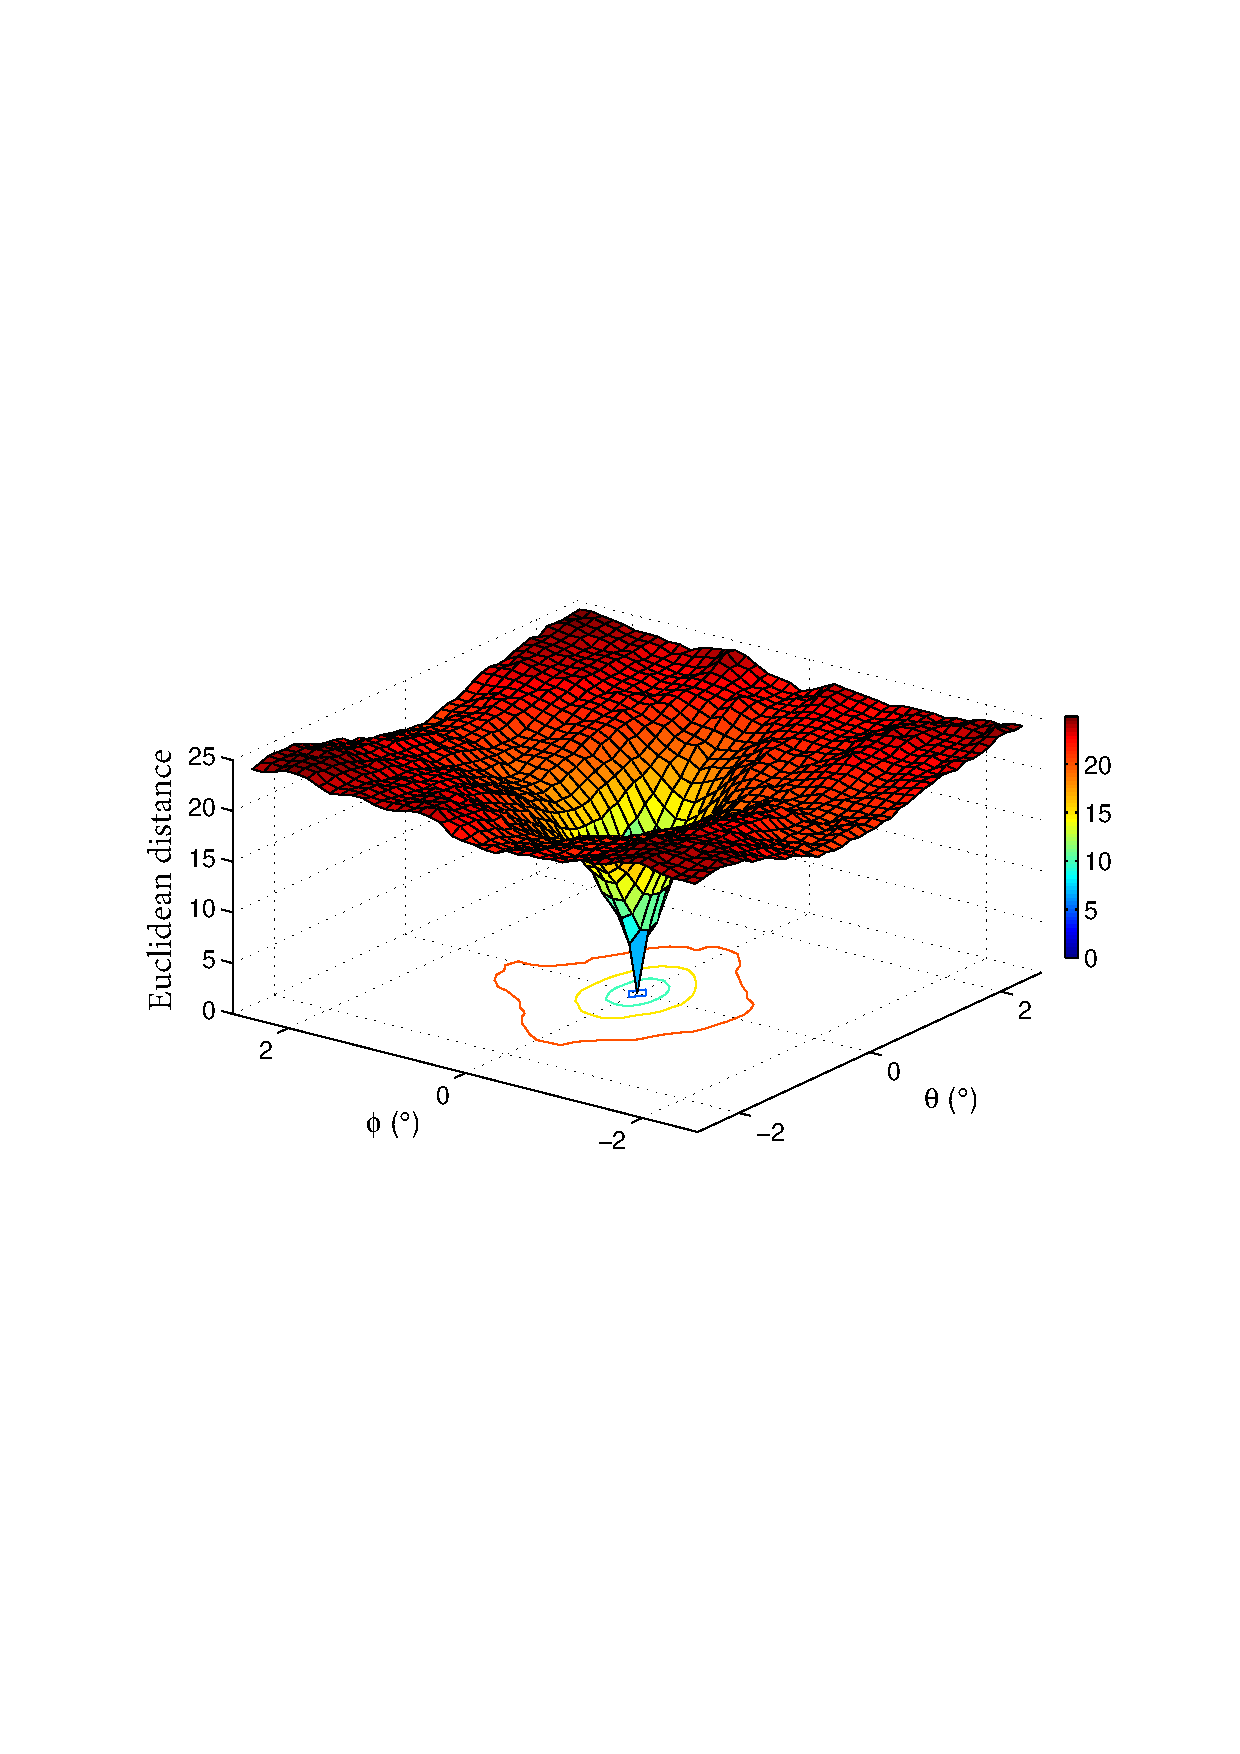
\includegraphics[width=8.0cm]{fig2_euc.pdf}}
    \caption{Euclidean distance between full-band RTF vectors as a function of the azimuth and elevation difference. See Section \ref{sec:expe} for the setup. One pose is fixed and the other is varied by up to $\pm 2.5^{\circ}$.}
    \label{fig2}
\end{figure}

\subsection{Network training}
\label{subsec:train}
During training, the networks are initialized following a standard procedure, i.e., the weights are initialized with Gaussian distributed samples and the biases with zeros. ReLU is used as the activation function for all the hidden layers and layer normalization~\cite{ba2016layer} is applied to regularize the parameters. The Adam method~\cite{kingma2014adam} is chosen to update the model using an adaptive learning rate.

One issue with the mini-batch based gradient descent is that the regularization in (\ref{eq:lossmr}) will tend to fail after random shuffling because of the sparse affinity inside the mini-batches, especially with large amount of training data. In~\cite{th2017acoustic}, a nearest-neighbor graph based solution was discussed to sample the data efficiently. We adopt a simpler technique here. The training samples are first randomly shuffled. We then start from one sample, collect all its neighbors, move on to the next remaining sample and repeat until the mini-batch size has been reached. The regularization is found to gradually take place against all the adjacent samples after several training epochs.


\section{Alternative decoder with regularization}
\label{sec:regul}

Given the locality property of the RTF manifold as discussed in Section \ref{subsec:manifold}, we are also motivated to apply regularization directly to the decoder. Similar to (\ref{eq:lossmr}), the loss function for the new decoder network can be defined by
\begin{equation}\label{eq:lossdr}
\sum_{i=1}^{L}\|\mathcal{D}({\bf p}_i)-{\bf h}_i\|^2 + \nu \sum_{i=1}^{L+U}\sum_{j=1}^{L+U}w_{ij}\|\mathcal{D}({\bf p}_i)-\mathcal{D}({\bf p}_j)\|^2
\end{equation}
where $\nu$ is a scaling factor, and the weight
\begin{equation}\label{eq:wij2}
  w_{ij} = \exp\left(-\frac{\|{\bf p}_i-{\bf p}_j\|^2}{\sigma^2}\right)
\end{equation}
depends on the distance between poses, with variance $\sigma^2$. Note that the loss function \eqref{eq:lossdr} doesn't depend on the unlabeled RTF samples anymore. Hence, arbitrarily many pose labels $\{{\bf p}_{L+1:L+U}\}$ can be defined without the need to collect unlabeled RTFs. This decoder is illustrated by Fig.~\ref{fig:dnn}(d).

\section{EXPERIMENTS AND ANALYSIS}
\label{sec:expe}
\subsection{Setup}

%The experiments are conducted in a simulated setup that is summarized in Table 1.

The experiments are conducted in a simulated room with $6\times 6.2\times 3$~m size and 300~ms reverberation time. Two omnidirectional microphones are positioned at $[3~3~1]$~m and $[3.2~3~1]$~m, respectively. The source is omnidirectional, hence the Euler angles $\alpha$, $\beta$, $\gamma$ are irrelevant and the notions of source pose and position are used interchangeably. The source position is confined to a spherical cap with radius $\rho=2$~m, azimuth $\theta \in [10^{\circ},60^{\circ}]$, and elevation $\phi \in [0^{\circ},30^{\circ}]$ with respect to the microphone pair, and it is sampled from a grid with $0.125^\circ$ stepsize in azimuth and elevation on this cap. \pfmarker{The setup here is similar to that in \cite{laufer2016mr} and \cite{deleforge2015acoustic}, which have been used to evaluate many studies in the field.} In total, there are $400\times 240$ poses.

For each pose, a 1~s white noise signal is emitted from the source and captured by the microphones. The sampling rate is 16~kHz. The corresponding acoustic impulses responses are simulated using an efficient implementation of the image-source method~\cite{rirge}. The STFT is applied with frame length 64~ms and 87.5\% overlap. The target RTF is then estimated as
\begin{equation}
\widehat{H}({\bf p}, k)=\frac{\sum_n A_2(n, k)A_1^*(n, k)}{\sum_n |A_1(n, k)|^2}
\end{equation}
with $*$ denoting complex conjugation and the full-band RTF vector is derived as in \eqref{eq:h}. Note that this estimator is one possible way to measure the RTF in real environments, and a white noise source signal \pfmarker{other than a speech signal}, provides a reliable estimation at all frequencies \cite{deleforge2015acoustic}. Among the training samples, 24 RTFs, that is only 0.025\% of the data, are labeled with their true source poses, creating a grid of 10$^\circ$ stepsize. We use two hidden layers with 1024 nodes each for the decoder and one hidden layer with 1024 nodes for the auxiliary encoder. The scaling factors $\lambda$, $\mu$, and $\nu$ are heuristically set to 0.01. The variances $\varsigma^2$ and $\sigma^2$ are set such that the weights of samples more than $2^\circ$ apart are close to 0.
%The development set? how to know when to stop training?

For evaluation, $T=1000$ extra poses are picked randomly on the same spherical cap. To our knowledge, there is no agreed-upon method to measure the closeness of two high-dimensional RTF vectors. We use the mean absolute error (MAE) to measure the prediction error at each frequency:
\begin{equation}\label{eq:err}
  \text{MAE} = \frac{1}{T}\sum_{t=1}^{T}|\widehat{\bf h}_t(k)-{\bf h}_t(k)|.
\end{equation}
The metric makes sense as we will show in Section \ref{subsec:further} by applying the predicted RTF to a speech enhancement task. The 95\% confidence interval (CI) on the MAE is also calculated to give an idea of the error distribution. The ILD and IPD prediction errors are treated separately. By IPD prediction error, we mean the error on the vector entries (sines and cosines) as in \eqref{eq:err}, not the angular error in radians.

\subsection{RTF inverse regression performance }

The prediction error of the three proposed models is shown in Fig.~3 for each frequency bin and the frequency averaged results are summarized in Table~1. For comparison, the free field model \eqref{eq:green} and a decoder trained using all $400\times 240$ labels are included as baselines.

\begin{figure}[tb]
    \centering
    \centerline{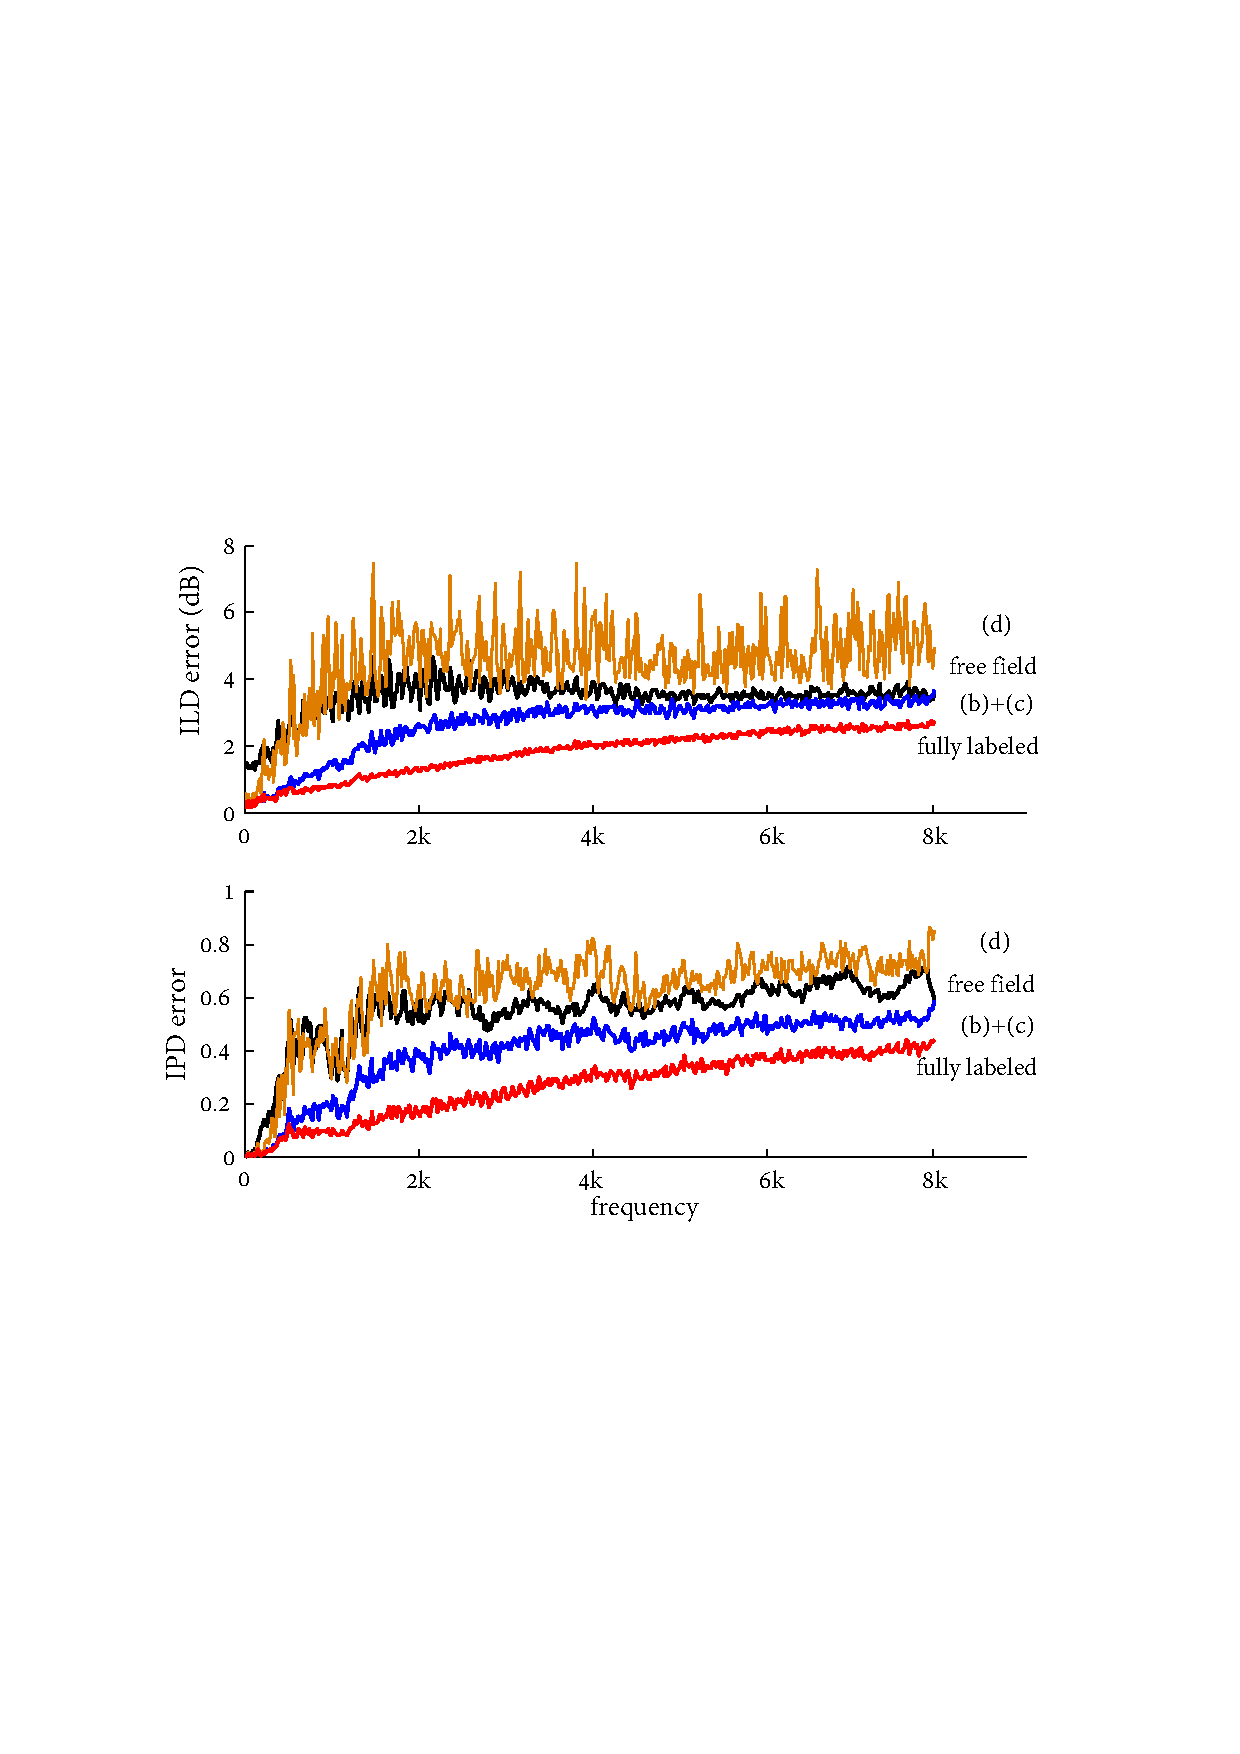
\includegraphics[width=8.5cm]{fig3_err_freq.pdf}}
    \caption{Mean absolute ILD/IPD prediction errors along frequency for network (d) (orange), the free field model \eqref{eq:green} (black), network (b)+(c) (blue), and the decoder trained with fully labeled data (red). \pfmarker{The results of network (a)+(c) are close to that of network (d) and are thus not shown for clearness.}}
    \label{fig3}
\end{figure}

The prediction errors clearly increase with frequency and become relatively stable at high frequencies. One possible reason could be that the RTFs vary more rapidly with respect to pose changes at high frequencies as can be concluded from the free field model (3), while the slow-varying RTFs at low frequencies are easier to be captured by the neural networks. The network trained with fully labeled data achieves the lowest mean prediction errors as expected, with 1.80$\pm$0.09 dB in ILD and 0.26$\pm$0.02 in IPD. It is largely better than other setups where only few training data are labeled. The unlabeled RTFs function differently in different architectures. The (b)+(c) network performs much better than the free field model, while the intuitive encoder-decoder setup (a)+(c), that relies on the same training data, fails to give good predictions.

To see how the unlabeled samples help, we investigate the localization performance achieved by the encoder networks by computing the root mean square error (RMSE) between the encoder outputs and the true source poses. For encoder (a), the localization RMSE is 13.08$^{\circ}$ in azimuth and 8.74$^{\circ}$ in elevation. For the encoder (b) with manifold regularization, the results are 2.94$^{\circ}$ and 2.08$^{\circ}$, respectively, which are quite accurate considering that the labeled samples are 10$^{\circ}$ apart. We can therefore interpret the encoders, and especially encoder (b), as providing the unlabeled RTFs with noisy pose labels. Additional experiments (not shown here) even indicate that encoder (b) slightly outperforms the recently proposed manifold regularization based localization method in \cite{laufer2016mr} on this data.

The decoder (d) with manifold regularization achieves a similar prediction error at frequencies below 1 kHz compared with the free-field model but its performance falls behind at high frequencies. This is not surprising since it does not make use of unlabeled RTFs.

%We conclude that the $l_2$ norm used to measure the affinity between RTFs in \eqref{eq:wij} is not proper since it ignores the angle of the high-dimensional vector, though the $l_2$ norm clearly makes more sense for measuring the poses.

% table
\begin{table}[tb]
\caption{Frequency averaged mean absolute ILD/IPD prediction errors (mean$\pm$CI bound) and SBF (dB).}
\label{table:1}
\begin{center}
\begin{tabular}{|l||c|c||c|}
  \hline
   Model               & ILD error & IPD error & SBF \\ \hline
   (a)+(c)    & 4.05$\pm$0.23 & 0.64$\pm$0.03  &  -0.60\\ \hline
   (d)        & 3.94$\pm$0.20 & 0.61$\pm$0.03   &  -0.35\\ \hline
   free field model & 3.47$\pm$0.16 & 0.55$\pm$0.03 & 0.69\\ \hline
   (b)+(c)    & 2.67$\pm$0.13 & 0.39$\pm$0.02    &  2.04   \\ \hline
   fully labeled & 1.80$\pm$0.09 & 0.26$\pm$0.02 &  3.19 \\ \hline
\end{tabular}
\end{center}
\end{table}

%\begin{figure}[tb]
%    \centering
%    \centerline{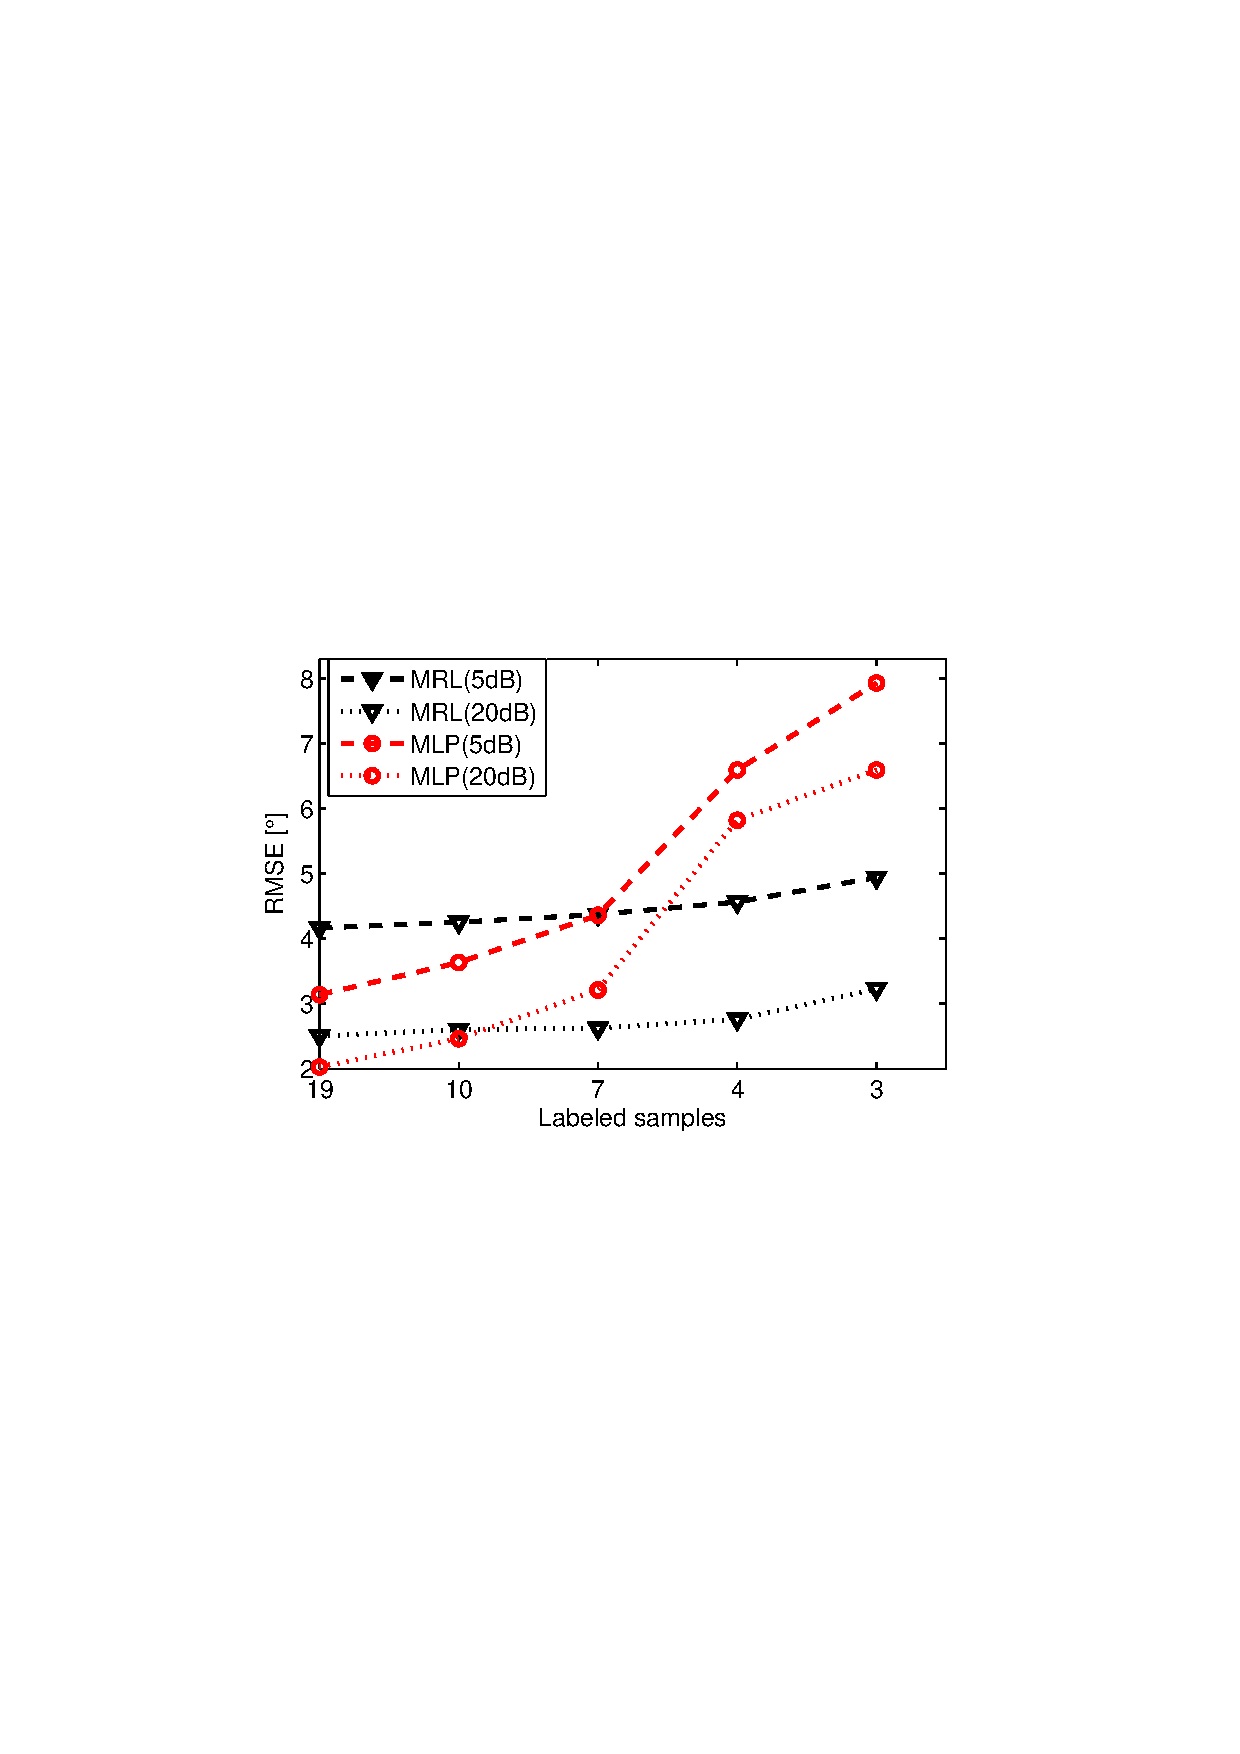
\includegraphics[width=8.0cm]{fig4_mrl.pdf}}
%    \caption{Localization RMSE of the encoder network (b) compared with MRL.}
%    \label{fig4}
%\end{figure}


\subsection{Further analysis}
\label{subsec:further}
It is commonly acknowledged that learning based methods would perform better with more training data and suffer performance loss in mismatched test conditions. These aspects are not further investigated here. Instead we evaluate the generated RTFs in a specific application, the generalized sidelobe canceler (GSC)~\cite{gannot2001signal}, that requires RTF in the implementation of a blocking matrix to provide the reference noise signal. We define the frequency-domain signal blocking factor (SBF) as
\begin{equation}\label{eq:sbf}
  \text{SBF}=10\log_{10}\frac{\sum_{n,k} \|A_1(n,k)\|^2}{\sum_{n,k} \|A_2(n,k)-H({\bf p},k)A_1(n,k)\|^2}
\end{equation}
where the denominator denotes the energy of the leakage signal. The SBF indicates the ability to block the first-channel source image in the second microphone and its value correlates negatively with signal distortion.

The SBF scores of different methods are given in Table~1. The results are consistent with the mean absolute prediction errors, with the fully labeled setup scoring the best (3.19 dB), the (b)+(c) network outperforming the free-field model, and the simple (a)+(c) the scoring the worst (-0.60 dB). Negative scores mean that the generated RTFs are not helpful at all.

The positive score achieved by the (b)+(c) network indicates that the predicted RTF can be considered as reliable prior information derived from the source pose. Further performance benefits are expected if this prior information is incorporated with the observations to achieve maximum a posteriori RTF estimation.


\section{CONCLUSIONS}
\label{sec:con}

We considered the RTF inverse regression task from a practical perspective where the training data are partially labeled and introduced a semi-supervised learning approach. Several possible neural network architectures were discussed. The proposed encoder with manifold regularization and decoder architecture outperformed the free-field model, in terms of both mean prediction error and signal blocking ability in the GSC application. Additional experiments showed that unlabeled RTFs and manifold regularization are both necessary to achieve good performance. Incorporating and evaluating the generated RTFs as prior information in other applications is worth further investigation in the future.


% Below is an example of how to insert images. Delete the ``\vspace'' line,
% uncomment the preceding line ``\centerline...'' and replace ``imageX.ps''
% with a suitable PostScript file name.
% -------------------------------------------------------------------------
%\begin{figure}[htb]

%\begin{minipage}[b]{1.0\linewidth}
%  \centering
%  \centerline{\includegraphics[width=8.5cm]{image1}}
%  \vspace{2.0cm}
%  \centerline{(a) Result 1}\medskip
%\end{minipage}
%
%\begin{minipage}[b]{.48\linewidth}
%  \centering
%  \centerline{\includegraphics[width=4.0cm]{image3}}
%  \vspace{1.5cm}
%  \centerline{(b) Results 3}\medskip
%\end{minipage}
%\hfill
%\begin{minipage}[b]{0.48\linewidth}
%  \centering
 % \centerline{\includegraphics[width=4.0cm]{image4}}
%  \vspace{1.5cm}
 % \centerline{(c) Result 4}\medskip
%\end{minipage}
%
%\caption{Example of placing a figure with experimental results.}
%\label{fig:res}
%
%\end{figure}


% To start a new column (but not a new page) and help balance the last-page
% column length use \vfill\pagebreak.
% -------------------------------------------------------------------------
%\vfill
%\pagebreak

%\section{COPYRIGHT FORMS}
%\label{sec:copyright}
%You must submit your fully completed, signed IEEE electronic copyright release
%form when you submit your paper. We {\bf must} have this form before your paper
%can be published in the proceedings.
%\vfill\pagebreak

%\newpage

% References should be produced using the bibtex program from suitable
% BiBTeX files (here: strings, refs, manuals). The IEEEbib.bst bibliography
% style file from IEEE produces unsorted bibliography list.
% -------------------------------------------------------------------------
\bibliographystyle{IEEEbib}
\bibliography{refs}

\end{document}
